\chapter{Modelling a Database for Dynamic Multimedia Data}

\todo[inline]{Is there more?}

\section{Adaptive Index Management}

\begin{figure}[h!]
    \centering
    \begin{subfigure}[b]{0.40\textwidth}
        \centering
        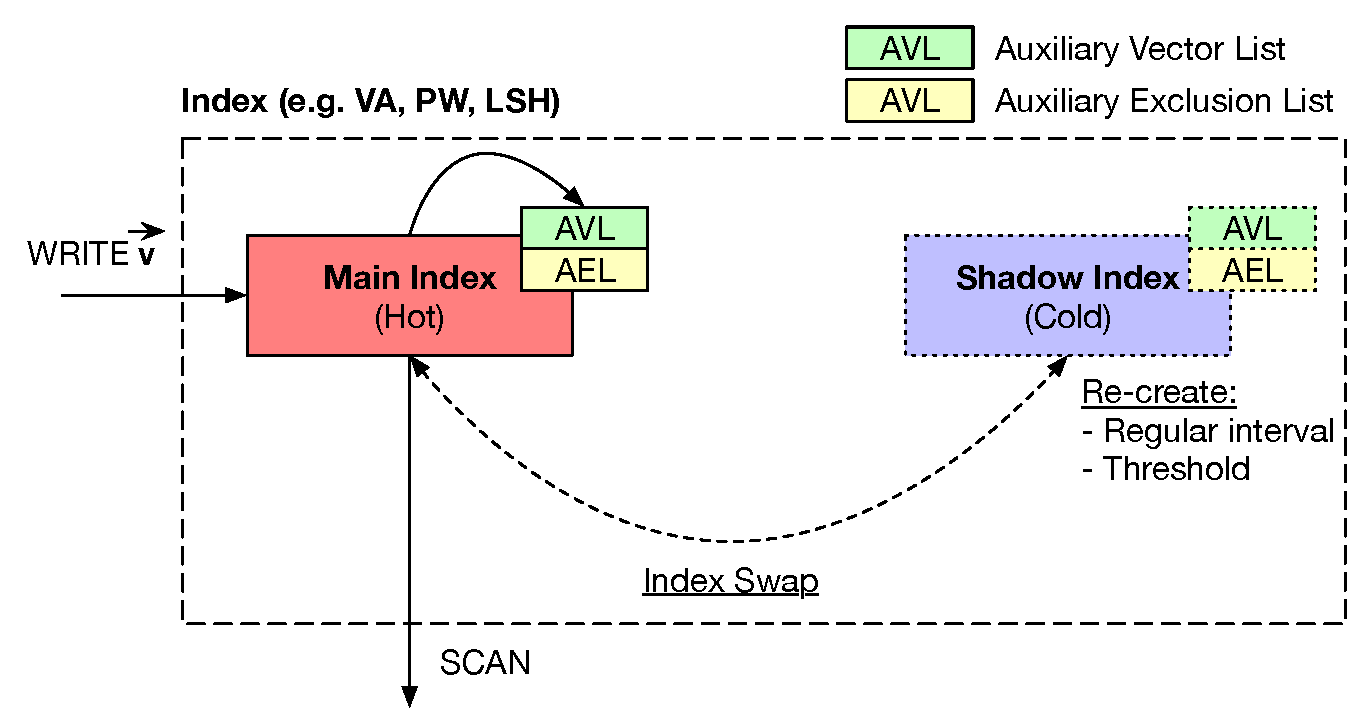
\includegraphics[width=\textwidth]{figures/adaptive_index.eps}
        \label{figure:adaptive_index}
    \end{subfigure}
    \hfill
    \begin{subfigure}[b]{0.40\textwidth}
        \centering
        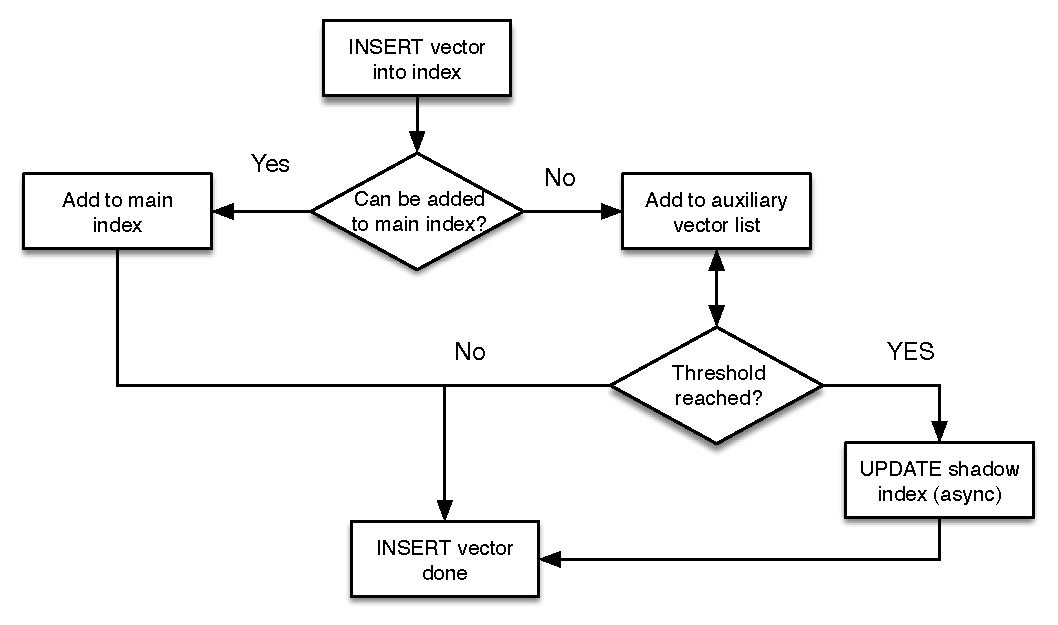
\includegraphics[width=\textwidth]{figures/adaptive_index_flow.eps}
        \label{figure:adaptive_index:flow}
    \end{subfigure}
    \label{fig:adaptive_index}
    \caption{Adaptive index structures overview.}
\end{figure}

Describe model for index management in the face of changing data (adaptive index management):

\begin{itemize}
    \item Reason about properties of secondary indexes for NNS (e.q., PQ, VA, LSH) with regards to data change
    \item Derivation of error bounds possible (e.g., usable for planning)?! Use in query planning?
    \item Systems perspective: How to cope with ``dirty'' indexes (e.g, auxilary data structure, offline optimization)
\end{itemize}

\section{Generalization of Similarity Search}

Describe generalized model for similarity search:

\begin{itemize}
    \item NNS: Scan -> (Predicate) -> Distance Function -> Sort -> Limit -> (Predicate); no need for dedicated language feature aside from distance function
    \item Distance function is a binary function $D(q,v) \longrightarrow d$ (consequence: different types of distance functions, application of weights merely an operation before executing the function etc.)
    \item $q$ and $v$ can be elements of $\mathbb{R}^d,\mathbb{C}^d$ or even matrices
    \item Systems perspective: How enable planner to reason about function execution
\end{itemize}

\section{Cost Model for Retrieval Accuracy}
Describe cost model with following properties:

\begin{itemize}
    \item Cost function: $f(a_{cpu}, a_{io}, a_{memory}, a_{accuracy}) \longrightarrow C$
    \item Means to estimate results accuracy from execution path (e.g., when using index) based on properties of the index
    \item Means to specify importance of accurate results (e.g., global, per-query, context-based i.e. when doing 1NN search) in comparison to other factors
    \item Cost usable in query planner
    \item What about execution time?
\end{itemize}

\section{Architecture Model}

\todo[inline]{Putting everything together into a unified systems model (base on previous work + aforementioned aspects).}




